% we will use beamer with
% a 16:9 aspect ratio
\documentclass[aspectratio=169]{beamer}

% font and input encodings
\usepackage[T1]{fontenc}
\usepackage[utf8]{inputenc}

% Fira Sans Light for the text
\usepackage[sfdefault,light]{FiraSans}

% since this is a tikzducks production,
% we have to load the package :)
\usepackage{tikzducks}

% the graphics package to
% include PDF assets
\usepackage{graphicx}

% disable navigation symbols, so
% we end up with a blank screen
\setbeamertemplate{navigation symbols}{}

\begin{document}

% no slide numbers
\pagestyle{empty}

% the following storyboard is inspired by
% the following YouTube video:
% youtube.com/watch?v=gG62zay3kck

% title
\begin{frame}{}
\centering

{\Huge Rhabarberbarbara\par}

\vspace{1em}

{\Large with Ti\emph{k}Zducks\par}

\end{frame}

% just Barbara
\begin{frame}{}

\hspace{4.5cm}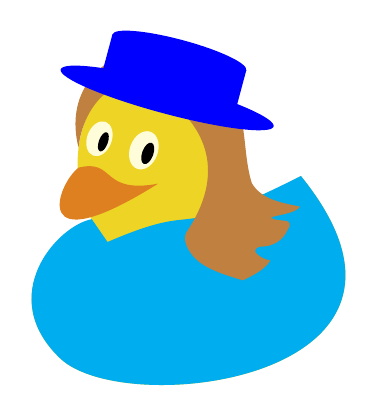
\begin{tikzpicture}[scale=2]
\duck[
  longhair,
  tshirt=cyan,
  hat=blue
]
\end{tikzpicture}

\begin{tikzpicture}[overlay]
\node at (10,4) {};
\end{tikzpicture}

\end{frame}

% Barbara + text
\begin{frame}{}

\hspace{4.5cm}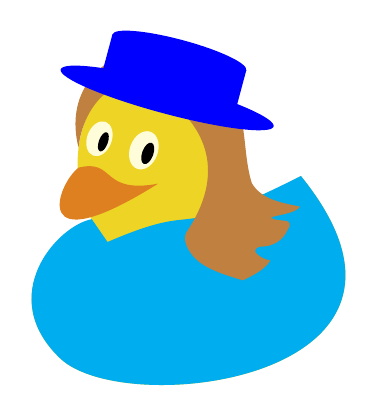
\begin{tikzpicture}[scale=2]
\duck[
  longhair,
  tshirt=cyan,
  hat=blue
]
\end{tikzpicture}

\begin{tikzpicture}[overlay]
\node at (10,4) {\LARGE Barbara};
\end{tikzpicture}

\end{frame}

% Barbara + cake + text
\begin{frame}{}

\hspace{4.5cm}\begin{tikzpicture}[scale=2]
\duck[
  longhair,
  tshirt=cyan,
  hat=blue
]

\node[xshift=-10] at (wing) {\includegraphics[scale=.1]{assets/cake}};
\end{tikzpicture}

\begin{tikzpicture}[overlay]
\node at (2.2,4) {\LARGE Rhabarberkuchen};
\end{tikzpicture}

\end{frame}

% Barbara + cake + text
\begin{frame}{}

\hspace{4.5cm}\begin{tikzpicture}[scale=2]
\duck[
  longhair,
  tshirt=cyan,
  hat=blue
]

\node[xshift=-10] at (wing) {\includegraphics[scale=.1]{assets/cake}};
\end{tikzpicture}

\begin{tikzpicture}[overlay]
\node at (6.5,-0.5) {\LARGE Rhabarberbarbara};
\end{tikzpicture}

\end{frame}

% Barbara + balloon text
\begin{frame}{}

\vspace*{-1.01cm}

\hspace{4.5cm}\begin{tikzpicture}[scale=2]
\duck[
  longhair,
  tshirt=cyan,
  hat=blue,
  think={\Huge\$\$\$}
]

\node[xshift=-10] at (wing) {\includegraphics[scale=.1]{assets/cake}};
\end{tikzpicture}

\begin{tikzpicture}[overlay]
\node at (10,4) {};
\end{tikzpicture}

\end{frame}

% bar asset
\begin{frame}{}

\hspace{3cm}\includegraphics[scale=.25]{assets/bar}

\begin{tikzpicture}[overlay]
\node at (7,5) {};
\end{tikzpicture}

\end{frame}

% bar asset + text
\begin{frame}{}

\hspace{3cm}\includegraphics[scale=.25]{assets/bar}

\begin{tikzpicture}[overlay]
\node at (7,5) {\LARGE Rhabarberbarbarabar};
\end{tikzpicture}

\end{frame}

% vikings
\begin{frame}{}

\hspace{4.5cm}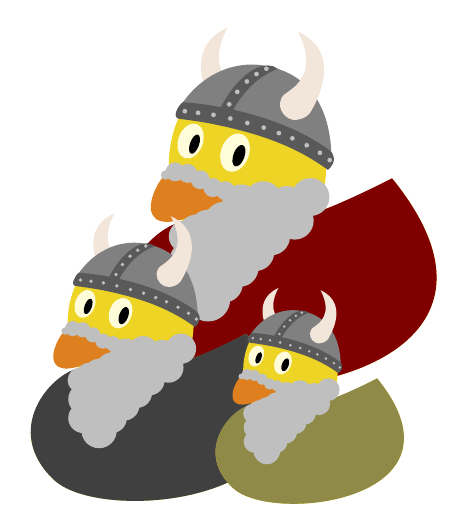
\begin{tikzpicture}[scale=2]
\duck[
  viking,
  tshirt=red!50!black,
  beard=gray!50!white
]

\duck[
  yshift=-20,
  scale=.8,
  xshift=-20,
  viking,
  tshirt=gray!50!black,
  beard=gray!50!white
]

\duck[
  yshift=-20,
  scale=.6,
  xshift=30,
  viking,
  tshirt=yellow!50!black,
  beard=gray!50!white
]
\end{tikzpicture}

\begin{tikzpicture}[overlay]
\node at (7,-0.5) {};
\end{tikzpicture}

\end{frame}

% vikings + text
\begin{frame}{}

\hspace{4.5cm}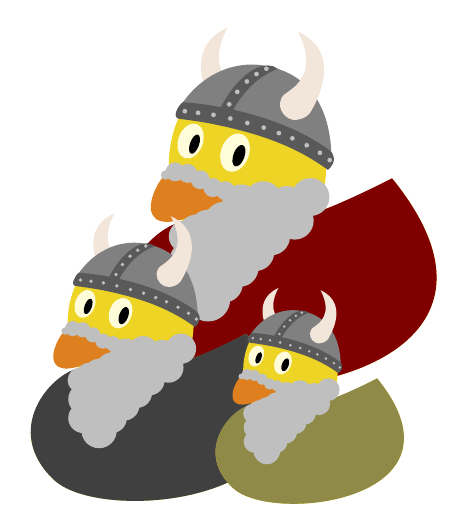
\begin{tikzpicture}[scale=2]
\duck[
  viking,
  tshirt=red!50!black,
  beard=gray!50!white
]

\duck[
  yshift=-20,
  scale=.8,
  xshift=-20,
  viking,
  tshirt=gray!50!black,
  beard=gray!50!white
]

\duck[
  yshift=-20,
  scale=.6,
  xshift=30,
  viking,
  tshirt=yellow!50!black,
  beard=gray!50!white
]
\end{tikzpicture}

\begin{tikzpicture}[overlay]
\node at (7,-0.5) {\LARGE Barbaren};
\end{tikzpicture}

\end{frame}

% bar asset + text
\begin{frame}{}

\hspace{3cm}\includegraphics[scale=.25]{assets/bar}

\begin{tikzpicture}[overlay]
\node at (7,5) {\LARGE Rhabarberbarbarabar};
\end{tikzpicture}

\end{frame}

% Barbara + text
\begin{frame}{}

\hspace{4.5cm}\begin{tikzpicture}[scale=2]
\duck[
  longhair,
  tshirt=cyan,
  hat=blue
]

\node[xshift=-10] at (wing) {\includegraphics[scale=.1]{assets/cake}};
\end{tikzpicture}

\begin{tikzpicture}[overlay]
\node at (6.5,-0.5) {\LARGE Rhabarberbarbara};
\end{tikzpicture}

\end{frame}

% Barbara + cake + text
\begin{frame}{}

\hspace{4.5cm}\begin{tikzpicture}[scale=2]
\duck[
  longhair,
  tshirt=cyan,
  hat=blue
]

\node[xshift=-10] at (wing) {\includegraphics[scale=.1]{assets/cake}};
\end{tikzpicture}

\begin{tikzpicture}[overlay]
\node at (2.2,4) {\LARGE Rhabarberkuchen};
\end{tikzpicture}

\end{frame}

% vikings + text
\begin{frame}{}

\hspace{4.5cm}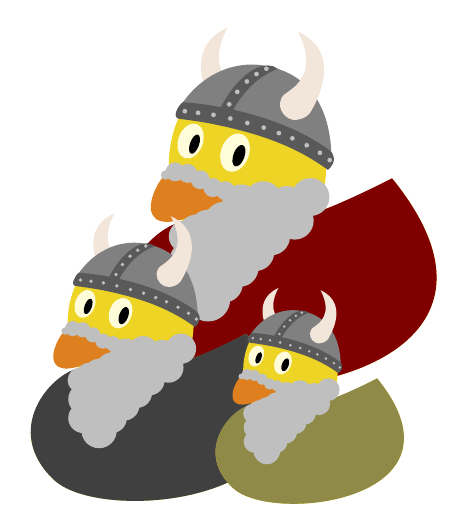
\begin{tikzpicture}[scale=2]
\duck[
  viking,
  tshirt=red!50!black,
  beard=gray!50!white
]

\duck[
  yshift=-20,
  scale=.8,
  xshift=-20,
  viking,
  tshirt=gray!50!black,
  beard=gray!50!white
]

\duck[
  yshift=-20,
  scale=.6,
  xshift=30,
  viking,
  tshirt=yellow!50!black,
  beard=gray!50!white
]
\end{tikzpicture}

\begin{tikzpicture}[overlay]
\node at (7,-0.5) {\LARGE Rhabarberbarbarabarbarbaren};
\end{tikzpicture}

\end{frame}

% vikings + beard text
\begin{frame}{}

\hspace{4.5cm}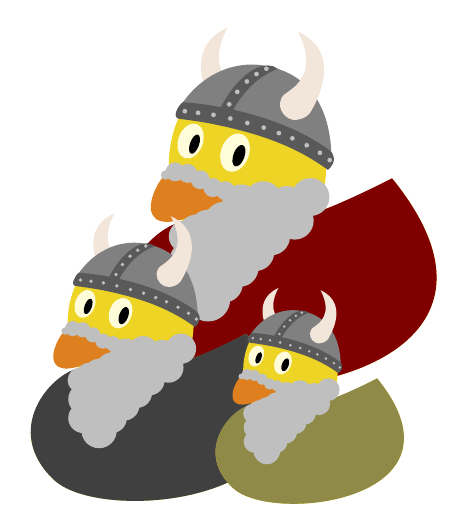
\begin{tikzpicture}[scale=2]
\duck[
  viking,
  tshirt=red!50!black,
  beard=gray!50!white
]

\duck[
  yshift=-20,
  scale=.8,
  xshift=-20,
  viking,
  tshirt=gray!50!black,
  beard=gray!50!white
]

\duck[
  yshift=-20,
  scale=.6,
  xshift=30,
  viking,
  tshirt=yellow!50!black,
  beard=gray!50!white
]
\end{tikzpicture}

\begin{tikzpicture}[overlay]
\node at (3.3,4) {\LARGE Bärte};
\end{tikzpicture}

\end{frame}

% vikings + text
\begin{frame}{}

\hspace{4.5cm}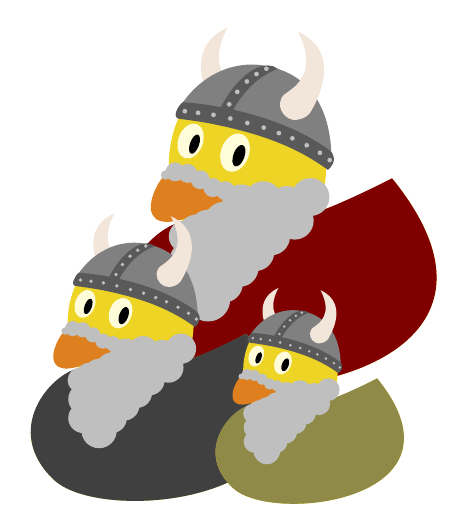
\begin{tikzpicture}[scale=2]
\duck[
  viking,
  tshirt=red!50!black,
  beard=gray!50!white
]

\duck[
  yshift=-20,
  scale=.8,
  xshift=-20,
  viking,
  tshirt=gray!50!black,
  beard=gray!50!white
]

\duck[
  yshift=-20,
  scale=.6,
  xshift=30,
  viking,
  tshirt=yellow!50!black,
  beard=gray!50!white
]
\end{tikzpicture}

\begin{tikzpicture}[overlay]
\node at (7,-0.5) {\LARGE Rhabarberbarbarabarbarbaren};
\end{tikzpicture}

\end{frame}

% vikings + beard text
\begin{frame}{}

\hspace{4.5cm}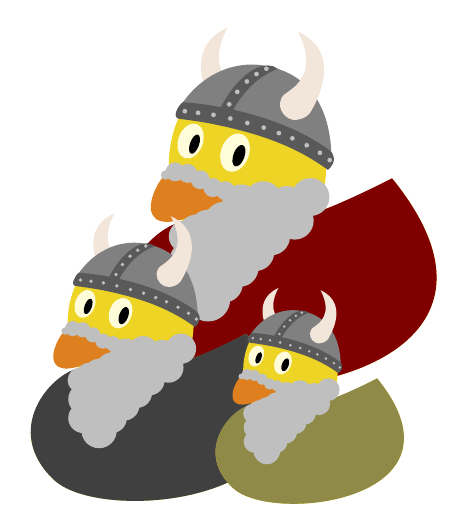
\begin{tikzpicture}[scale=2]
\duck[
  viking,
  tshirt=red!50!black,
  beard=gray!50!white
]

\duck[
  yshift=-20,
  scale=.8,
  xshift=-20,
  viking,
  tshirt=gray!50!black,
  beard=gray!50!white
]

\duck[
  yshift=-20,
  scale=.6,
  xshift=30,
  viking,
  tshirt=yellow!50!black,
  beard=gray!50!white
]
\end{tikzpicture}

\begin{tikzpicture}[overlay]
\node at (7,-0.5) {\LARGE Rhabarberbarbarabarbarbarenbärte};
\end{tikzpicture}

\end{frame}

% barber + text
\begin{frame}{}

\hspace{6cm}\begin{tikzpicture}[scale=2]
\duck[
  shorthair=black,
  tshirt,
  jacket=gray,
  tie=cyan,
  glasses=red!50!black
]

\node[xshift=-30] at (wing) {\includegraphics[scale=.3]{assets/scissors}};
\end{tikzpicture}

\begin{tikzpicture}[overlay]
\node at (11,4) {\LARGE Barbier};
\end{tikzpicture}

\end{frame}

% viking + beard text
\begin{frame}{}

\hspace{4.5cm}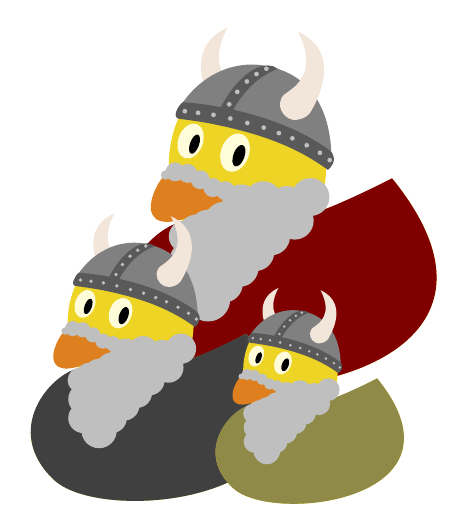
\begin{tikzpicture}[scale=2]
\duck[
  viking,
  tshirt=red!50!black,
  beard=gray!50!white
]

\duck[
  yshift=-20,
  scale=.8,
  xshift=-20,
  viking,
  tshirt=gray!50!black,
  beard=gray!50!white
]

\duck[
  yshift=-20,
  scale=.6,
  xshift=30,
  viking,
  tshirt=yellow!50!black,
  beard=gray!50!white
]
\end{tikzpicture}

\begin{tikzpicture}[overlay]
\node at (7,-0.5) {\LARGE Rhabarberbarbarabarbarbarenbart};
\end{tikzpicture}

\end{frame}

% barber + text
\begin{frame}{}

\hspace{6cm}\begin{tikzpicture}[scale=2]
\duck[
  shorthair=black,
  tshirt,
  jacket=gray,
  tie=cyan,
  glasses=red!50!black
]

\node[xshift=-30] at (wing) {\includegraphics[scale=.3]{assets/scissors}};
\end{tikzpicture}

\begin{tikzpicture}[overlay]
\node at  (7,-0.5) {\LARGE Rhabarberbarbarabarbarbarenbartbarbier};
\end{tikzpicture}

\end{frame}

% bar asset
\begin{frame}{}

\hspace{3cm}\includegraphics[scale=.25]{assets/bar}

\begin{tikzpicture}[overlay]
\node at (7,5) {\LARGE Rhabarberbarbarabar};
\end{tikzpicture}

\end{frame}

% Barbara + text
\begin{frame}{}

\hspace{4.5cm}\begin{tikzpicture}[scale=2]
\duck[
  longhair,
  tshirt=cyan,
  hat=blue
]

\node[xshift=-10] at (wing) {\includegraphics[scale=.1]{assets/cake}};
\end{tikzpicture}

\begin{tikzpicture}[overlay]
\node at (6.5,-0.5) {\LARGE Rhabarberbarbara};
\end{tikzpicture}

\end{frame}

% Barbara + cake + text
\begin{frame}{}

\hspace{4.5cm}\begin{tikzpicture}[scale=2]
\duck[
  longhair,
  tshirt=cyan,
  hat=blue
]

\node[xshift=-10] at (wing) {\includegraphics[scale=.1]{assets/cake}};
\end{tikzpicture}

\begin{tikzpicture}[overlay]
\node at (2.2,4) {\LARGE Rhabarberkuchen};
\end{tikzpicture}

\end{frame}

% barber + beer asset
\begin{frame}{}

\vspace*{-.2cm}

\hspace{2.7cm}\includegraphics[scale=.35]{assets/beer}
\hspace{1em}
\begin{tikzpicture}[scale=2]
\duck[
  shorthair=black,
  tshirt,
  jacket=gray,
  tie=cyan,
  glasses=red!50!black
]

\node[xshift=-30] at (wing) {\includegraphics[scale=.3]{assets/scissors}};
\end{tikzpicture}

\begin{tikzpicture}[overlay]
\node at  (3,4) {};
\end{tikzpicture}

\end{frame}

% barber + beer text
\begin{frame}{}

\vspace*{-.2cm}

\hspace{2.7cm}\includegraphics[scale=.35]{assets/beer}
\hspace{1em}
\begin{tikzpicture}[scale=2]
\duck[
  shorthair=black,
  tshirt,
  jacket=gray,
  tie=cyan,
  glasses=red!50!black
]

\node[xshift=-30] at (wing) {\includegraphics[scale=.3]{assets/scissors}};
\end{tikzpicture}

\begin{tikzpicture}[overlay]
\node at  (3,4) {\Large Bier};
\end{tikzpicture}

\end{frame}

% barber + text
\begin{frame}{}

\vspace*{-.2cm}

\hspace{2.7cm}\includegraphics[scale=.35]{assets/beer}
\hspace{1em}
\begin{tikzpicture}[scale=2]
\duck[
  shorthair=black,
  tshirt,
  jacket=gray,
  tie=cyan,
  glasses=red!50!black
]

\node[xshift=-30] at (wing) {\includegraphics[scale=.3]{assets/scissors}};
\end{tikzpicture}

\begin{tikzpicture}[overlay]
\node at  (7,-0.5) {\LARGE Rhabarberbarbarabarbarbarenbartbarbierbier};
\end{tikzpicture}

\end{frame}

% bar asset + Bärbel
\begin{frame}{}

\hspace{3cm}\includegraphics[scale=.25]{assets/bar}

\hspace{10cm}\begin{tikzpicture}[scale=1.5, overlay]
\duck[
  longhair=red!70!black,
  tshirt,
  jacket=gray!50!black,
  bowtie
]
\end{tikzpicture}

\begin{tikzpicture}[overlay]
\node at (7,5) {};
\end{tikzpicture}

\end{frame}

% barber + beer + text
\begin{frame}{}

\vspace*{-.2cm}

\hspace{2.7cm}\includegraphics[scale=.35]{assets/beer}
\hspace{1em}
\begin{tikzpicture}[scale=2]
\duck[
  shorthair=black,
  tshirt,
  jacket=gray,
  tie=cyan,
  glasses=red!50!black
]

\node[xshift=-30] at (wing) {\includegraphics[scale=.3]{assets/scissors}};
\end{tikzpicture}

\begin{tikzpicture}[overlay]
\node at  (7,-0.5) {\LARGE Rhabarberbarbarabarbarbarenbartbarbierbier};
\end{tikzpicture}

\end{frame}

% bar asset + Bärbel + text
\begin{frame}{}

\hspace{3cm}\includegraphics[scale=.25]{assets/bar}

\hspace{10cm}\begin{tikzpicture}[scale=1.5, overlay]
\duck[
  longhair=red!70!black,
  tshirt,
  jacket=gray!50!black,
  bowtie
]
\end{tikzpicture}

\begin{tikzpicture}[overlay]
\node at (7,5.5) {\LARGE Rhabarberbarbarabarbarbarenbartbarbierbierbar};
\end{tikzpicture}

\end{frame}

% bar asset + Bärbel + text
\begin{frame}{}

\hspace{3cm}\includegraphics[scale=.25]{assets/bar}

\hspace{10cm}\begin{tikzpicture}[scale=1.5, overlay]
\duck[
  longhair=red!70!black,
  tshirt,
  jacket=gray!50!black,
  bowtie
]
\end{tikzpicture}

\begin{tikzpicture}[overlay]
\node at (12.5,4.5) {\LARGE Bärbel};
\end{tikzpicture}

\end{frame}

% vikings + text
\begin{frame}{}

\hspace{4.5cm}\begin{tikzpicture}[scale=2]
\duck[
  viking,
  tshirt=red!50!black,
  beard=gray!50!white
]

\duck[
  yshift=-20,
  scale=.8,
  xshift=-20,
  viking,
  tshirt=gray!50!black,
  beard=gray!50!white
]

\duck[
  yshift=-20,
  scale=.6,
  xshift=30,
  viking,
  tshirt=yellow!50!black,
  beard=gray!50!white
]
\end{tikzpicture}

\begin{tikzpicture}[overlay]
\node at (7,-0.5) {\LARGE Rhabarberbarbarabarbarbaren};
\end{tikzpicture}

\end{frame}

% barber + text
\begin{frame}{}

\vspace*{-.2cm}

\hspace{2.7cm}\includegraphics[scale=.35]{assets/beer}
\hspace{1em}
\begin{tikzpicture}[scale=2]
\duck[
  shorthair=black,
  tshirt,
  jacket=gray,
  tie=cyan,
  glasses=red!50!black
]

\node[xshift=-30] at (wing) {\includegraphics[scale=.3]{assets/scissors}};
\end{tikzpicture}

\begin{tikzpicture}[overlay]
\node at  (7,-0.5) {\LARGE Rhabarberbarbarabarbarbarenbartbarbier};
\end{tikzpicture}

\end{frame} 

% bar asset + Bärbel + text
\begin{frame}{}

\hspace{3cm}\includegraphics[scale=.25]{assets/bar}

\hspace{10cm}\begin{tikzpicture}[scale=1.5, overlay]
\duck[
  longhair=red!70!black,
  tshirt,
  jacket=gray!50!black,
  bowtie
]
\end{tikzpicture}

\begin{tikzpicture}[overlay]
\node at (7,5.5) {\LARGE Rhabarberbarbarabarbarbarenbartbarbierbierbarbärbel};
\end{tikzpicture}

\end{frame}

% bar asset + text
\begin{frame}{}

\hspace{3cm}\includegraphics[scale=.25]{assets/bar}

\hspace{10cm}\begin{tikzpicture}[scale=1.5, overlay]

\end{tikzpicture}

\begin{tikzpicture}[overlay]
\node at (7,5.5) {\LARGE Rhabarberbarbarabar};
\end{tikzpicture}

\end{frame}

% Barbara + text
\begin{frame}{}

\hspace{4.5cm}\begin{tikzpicture}[scale=2]
\duck[
  longhair,
  tshirt=cyan,
  hat=blue
]

\node[xshift=-10] at (wing) {\includegraphics[scale=.1]{assets/cake}};
\end{tikzpicture}

\begin{tikzpicture}[overlay]
\node at (6.5,-0.5) {\LARGE Rhabarberbarbara};
\end{tikzpicture}

\end{frame}

% Barbara + cake + text
\begin{frame}{}

\hspace{4.5cm}\begin{tikzpicture}[scale=2]
\duck[
  longhair,
  tshirt=cyan,
  hat=blue
]

\node[xshift=-10] at (wing) {\includegraphics[scale=.1]{assets/cake}};
\end{tikzpicture}

\begin{tikzpicture}[overlay]
\node at (2.2,4) {\LARGE Rhabarberkuchen};
\end{tikzpicture}

\end{frame}

% barber + beer + text
\begin{frame}{}

\vspace*{-.2cm}

\hspace{2.7cm}\includegraphics[scale=.35]{assets/beer}
\hspace{1em}
\begin{tikzpicture}[scale=2]
\duck[
  shorthair=black,
  tshirt,
  jacket=gray,
  tie=cyan,
  glasses=red!50!black
]

\node[xshift=-30] at (wing) {\includegraphics[scale=.3]{assets/scissors}};
\end{tikzpicture}

\begin{tikzpicture}[overlay]
\node at  (7,-0.5) {\LARGE Rhabarberbarbarabarbarbarenbartbarbierbier};
\end{tikzpicture}

\end{frame} 

% cheers!
\begin{frame}{}
\centering\Huge

Prost!

\end{frame}

% woo

\end{document}
